
\resetcounters
\bibliographystyle{asp2010}

\markboth{Landais, Ochsenbein, and Simon}{TAPVizieR: A New Way to Access the \ssindex{catalogs!services!VizieR}\ssindex{databases!individual!VizieR}VizieR Database}

\resetcounters

\title{TAP\ssindex{catalogs!services!VizieR}\ssindex{databases!individual!VizieR}VizieR: A New Way to Access the \ssindex{databases!individual!VizieR}VizieR Database}
\author{Gilles~Landais, Fran\c cois~Ochsenbein, Anne-Camille~Simon
\affil{Centre de Donn\'ees astronomiques de Strasbourg (CDS) }}

\aindex{Landais, G.}
\aindex{Ochsenbein, F.}
\aindex{Simon, A.-C.}

\begin{abstract}
\ssindex{catalogs!services!VizieR}\ssindex{databases!individual!VizieR}VizieR is a component of the \ssindex{Virtual Observatory (VO)}Virtual Observatory: it provides tables of catalogs to external software with\ssindex{Virtual Observatory(VO)} VO standards like the \ssindex{data formats!VOTable}VOTable output. Accessing \ssindex{catalogs!services!VizieR}VizieR with the \ssindex{databases!querylanguage!ADQL}ADQL/\ssindex{protocols!TAP}TAP standard represents a new milestone in the \ssindex{catalogs!services!VizieR}\ssindex{databases!individual!VizieR}VizieR access facilities.

The \ssindex{databases!Postgres}PostgreSQL engine has been chosen to store data: it provides a solid database containing utilities to manage\ssindex{databases!querylanguage!SQL} SQL or to create the customized \ssindex{libraries!HEALPix}HEALPix\ooindex{HEALPix, ascl:1107.018} indexing ``\ssindex{methods!indexing!H3C}H3C'' which permits fast access from sky coordinates. The \ssindex{protocols!TAP}TAP standard however was not designed to accommodate databases managing tens of thousands of tables like \ssindex{catalogs!services!VizieR}VizieR, and some compromises with the \ssindex{protocols!TAP}TAP standard were necessary in this first version of TAPVizieR.
\end{abstract}

\section{The context}

\ssindex{databases!querylanguage!ADQL}ADQL \citep{adql_2011} is an other way to query \ssindex{catalogs!services!VizieR}\ssindex{databases!individual!VizieR}VizieR tables \citep{ochsenbein_2000}; \ssindex{databases!querylanguage!ADQL}ADQL is an extension of\ssindex{databases!querylanguage!SQL} SQL with additional astronomical functions and geometrical objects. It enables the usage of formulae involving column combinations which can be used for display or to filter a set of records (see Figure~\ref{P044:ADQLexample}). These kinds of operations were limited in the \ssindex{catalogs!services!VizieR}\ssindex{databases!individual!VizieR}VizieR application and required the usage of external software for such computations.

\begin{figure}[!h] \center
\begin{footnotesize}
\begin{verbatim}
SELECT ra_icrs_, de_icrs_, BTmag-VTmag as B-V
FROM   tyc2
WHERE  1=CONTAINS(POINT('ICRS', ra_icrs_, de_icrs_),
                  CIRCLE('ICRS', 244.26, -22.98, 10/60.))
   AND BTmag-VTmag<1
\end{verbatim}\end{footnotesize}
\caption{Example of an \ssindex{databases!querylanguage!ADQL}ADQL query on the catalog Tycho using a color constraint (BTmag-VTmag) and a cone search arround M80.}\label{P044:ADQLexample}
\end{figure}

\ssindex{protocols!TAP}TAP \citep{tap_2011} is a protocol to execute an \ssindex{databases!querylanguage!ADQL}ADQL query on a remote database. \ssindex{protocols!TAP}TAP services are already available in data centers like \ssindex{data centers!Canadian Astronomy Data Centre (CADC)}CADC or \ssindex{data centers!GAVO}GAVO, and some external software like \ssindex{applications!TOPCAT}TOPCat\ooindex{TOPCAT, ascl:1101.010} or \ssindex{applications!TapHandle}TAPHandle can work with the standard. These applications link tables coming from different databases (\ssindex{data centers!GAVO}\ssindex{Virtual Observatory (VO)!individual!German Astrophysical Virtual Observatory (GAVO)}GAVO, \ssindex{data centers!Canadian Astronomy Data Centre (CADC)}CADC and now \ssindex{catalogs!services!VizieR}\ssindex{databases!individual!VizieR}VizieR) with a unique interface and use the same language. They offer real extended possibilities for astronomers who can combine tables stored in different places.


\section{A Dedicated Database}

\subsection{Homogenize the Storage}
The \ssindex{catalogs!services!VizieR}VizieR application provides catalogs. The tables and their \ssindex{data!metadata}metadata (descriptions) are stored in a transactionnal database, or in dedicated binary files for the large catalogs (e.g. \ssindex{observatories!space-based!WISE}WISE, \ssindex{observatories!Earth-based!2MASS}2MASS, \ssindex{surveys!Sloan Digital Sky Survey(SDSS)}SDSS, etc.) in order to speed up the search by position.

\ssindex{databases!querylanguage!ADQL}ADQL based on\ssindex{databases!querylanguage!SQL} SQL requires a transactional database or technologies like \ssindex{packages!Hadoop}Hadoop. We think that\ssindex{databases!querylanguage!SQL} SQL is the more practical way to be \ssindex{databases!querylanguage!ADQL}ADQL-compatible, so, we chose to create a new dedicated database which gathers all catalogs. 

This new database is a \ssindex{databases!Postgres}PostgreSQL engine which effectively supports 3.5 Tb of data and indexes. With \ssindex{databases!Postgres}PostgreSQL, we gain the replication capabilities and some easy way to create advanced functions.

\subsection{Indexation}
\ssindex{catalogs!services!VizieR}\ssindex{databases!individual!VizieR}VizieR has tables that can contain up to 1 billion records. This volumetry needs indexation and in particular a positional indexation, because conesearch or crossmatch (join tables according to their positions) are the most popular functionalities in \ssindex{catalogs!services!VizieR}\ssindex{databases!individual!VizieR}VizieR.

In \ssindex{databases!Postgres}PostgreSQL an index by position can be built with libraries like \ssindex{methods!indexing!PgSphere}\ssindex{libraries!PgSphere}PgSphere provided by \ssindex{databases!Postgres}PostgreSQL; an external plugin \ssindex{methods!indexing!Q3C}Q3C was also developed by \citet{q3c_2006} for astronomical applications. The \ssindex{methods!indexing!PgSphere}\ssindex{libraries!PgSphere}PgSphere is user-friendly; however, \ssindex{methods!indexing!Q3C}Q3C minimizes resources and is more efficient with tables containing over one million records --- therefore better suited for \ssindex{catalogs!services!VizieR}\ssindex{databases!individual!VizieR}VizieR. \ssindex{methods!indexing!Q3C}Q3C works with the quadcube algorithm; however, {\em \ssindex{libraries!HEALPix}HEALPix}\ooindex{HEALPix, ascl:1107.018} is more and more becoming a standard in astronomical applications like \ssindex{applications!Aladin}Aladin\ooindex{Aladin, ascl:1112.019}, the CDS Crossmatch service, \ssindex{observatories!space-based!Gaia}GAIA, etc.


\paragraph{The \ssindex{methods!indexing!H3C}H3C library}

We built a 2D PostgreSQL library \textbf{H3C} (\textit{i.e. \textbf{H}ealpiX-\textbf{T}ree-C code}), largely inspired from  \ssindex{methods!indexing!Q3C}Q3C, with the same functionalities --- with the exception that the functions dealing with polygons are available for convexes only.

The \ssindex{methods!tessellation}tessellation of the sphere with \ssindex{libraries!HEALPix}HEALPix\ooindex{HEALPix, ascl:1107.018} cells requires however a deep resolution to be as efficient as \ssindex{methods!indexing!Q3C}Q3C. This implementation was possible thanks to the recent improvement of the  \ssindex{libraries!HEALPix}HEALPix\ooindex{HEALPix, ascl:1107.018}\ssindex{computing!architecture} 64bits \ssindex{computer languages!C++}C++ library maintained by NASA \citep{gorski_healpix}.

\paragraph{Some comparisons between libraries} (see Figure~\ref{P044:comparative}) Regarding  efficiency, the tests show that \ssindex{methods!indexing!Q3C}Q3C and \ssindex{methods!indexing!H3C}H3C are largely better than \ssindex{methods!indexing!PgSphere}\ssindex{libraries!PgSphere}PgSphere. Moreover the size required by the index as well as the time required for their creation, are significantly smaller with \ssindex{methods!indexing!Q3C}Q3C/\ssindex{methods!indexing!H3C}H3C than with \ssindex{methods!indexing!PgSphere}\ssindex{libraries!PgSphere}PgSphere.

\begin{figure}[htp] \center
\begin{small}
\begin{tabular}{lllll}
 & \ssindex{methods!indexing!PgSphere}\ssindex{libraries!PgSphere}PgSphere & \ssindex{methods!indexing!Q3C}Q3C & \ssindex{methods!indexing!H3C}H3C & H3C  \\
 &          &     &     &{\scriptsize cluster index} \\
conesearch in 2mass (M1, radius:2arcsec) & 340ms& 360ms& 380ms &\\
conesearch in 2mass (M1, radius:2arcmin) & 500ms& 390ms& 400ms &\\
conesearch in 2mass (M1, radius:2deg)    & 88s& 4.3s& 1.26s &\\
crossmatch Tycho-\ssindex{observatories!space-based!Hipparcos}hipparcos & 110s & 4.5s &  4.5s & 3s\\ 
crossmatch \ssindex{observatories!Earth-based!2MASS}2mass-\ssindex{observatories!space-based!Hipparcos}hipparcos & 48min & 15min & 14min & 6.5min\\ 
crossmatch \ssindex{observatories!Earth-based!2MASS}2mass-Tycho     & 4h30 & 49min  & 48min & 11.5min\\ 
\end{tabular}
\end{small}
\caption{Comparisons of the positional indexation applied to \ssindex{observatories!space-based!Hipparcos}Hipparcos ($\sim$100K records), Tycho ($\sim$2.5M records) and \ssindex{catalogs!individual!2MASS}2mass ($\sim$450M records) catalogues. All tests are performed on the same Linux computer (99G RAM) using a \ssindex{databases!Postgres}PostgreSQL (version 9.1) database. The cache disk was deleted before each test.}
\label{P044:comparative}
\end{figure}

\paragraph{Managing the coordinate systems}

The coordinate system used in \ssindex{catalogs!services!VizieR}\ssindex{databases!individual!VizieR}VizieR tables depends on the catalog, but \ssindex{catalogs!services!VizieR}\ssindex{databases!individual!VizieR}VizieR can compute positions of any catalog in another coordinate system than the original one, taking into account the \ssindex{astronomy!proper motion}proper motions when these are described in the \ssindex{catalogs!services!VizieR}VizieR METAdata.

Working with a unique coordinate system is obviously more efficient in \ssindex{databases!querylanguage!ADQL}ADQL, especially for crossmatches. So, we are adding the position in the ICRS frame in each table; the new columns (\_ra.icrs, \_de.icrs) are computed for the epoch J2000 if \ssindex{astronomy!proper motion}proper motions are known.


\section{TAPVizieR Implementation}

\subsection{Technologies and the Library Used}
\paragraph{The database}


The TAPVizieR service uses a \ssindex{databases!Postgres}PostgreSQL database and takes advantage of the C-functions to index positions using \ssindex{methods!indexing!H3C}H3C;  functions dealing with coordinate conversions were also added on the server side.

\paragraph{Parsing the \ssindex{databases!querylanguage!ADQL}ADQL query and providing data with \ssindex{protocols!TAP}TAP}

The \ssindex{protocols!TAP}TAP/\ssindex{databases!querylanguage!ADQL}ADQL service is a Web\ssindex{web!applications} application written in \ssindex{computer languages!Java}Java. We use the \ssindex{protocols!UWS}UWS/\ssindex{protocols!TAP}TAP and \ssindex{databases!querylanguage!ADQL}ADQL libraries \citep{simbad_tap_2011}, which were helpful in translating \ssindex{databases!querylanguage!ADQL}ADQL into an object tree to easily handle the \ssindex{catalogs!services!VizieR}VizieR METAdata. 

\paragraph{Architecture}
The TAPVizieR architecture is composed of the \ssindex{protocols!TAP}TAP/\ssindex{databases!querylanguage!ADQL}ADQL web\ssindex{web!applications} application, a \ssindex{databases!individual!VizieR}VizieR mirror and a \ssindex{databases!Postgres}PostgreSQL installation (see Figure~\ref{P044:architecture}). The database is composed of a master and a standby database using the synchronous replication available in \ssindex{databases!Postgres}PostgreSQL since version 9.1. The pool {\em PgBouncer} is also used to manage database connections, and to enable a precise configuration. 

\begin{figure}[hbp] \center
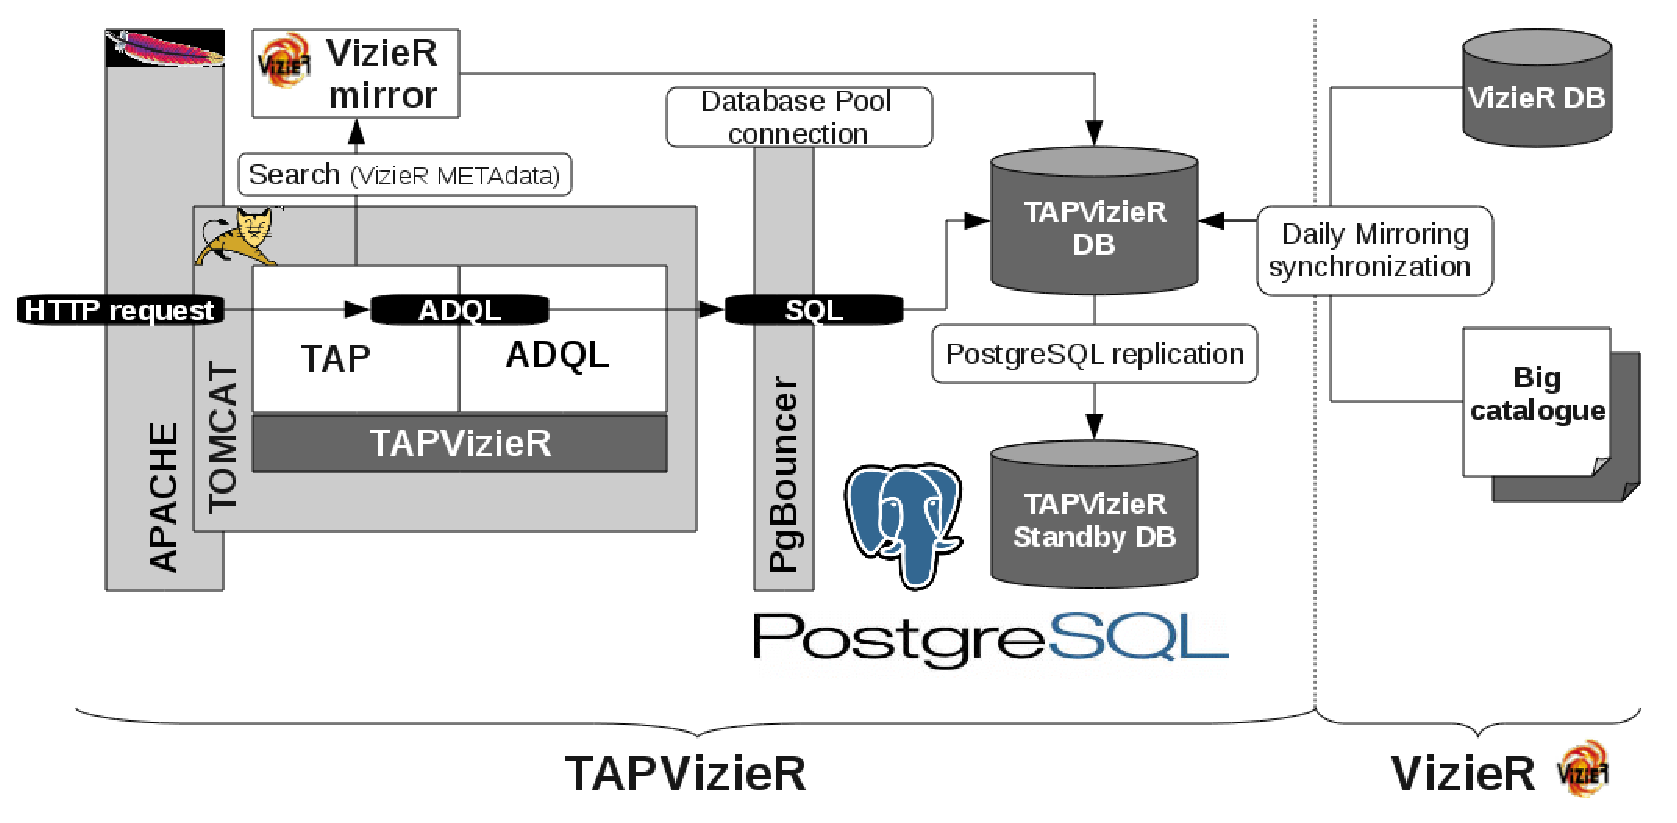
\includegraphics[width=0.85\textwidth]{part8/Landais_P44/P044_fig1.eps}
\caption{The TAPVizieR architecture}\label{P044:architecture}
\end{figure}

\subsection{The Web interface}
\label{P044:web_interface}
Two modes are available to query tables in TAPVizieR. The first, the {\em \ssindex{protocols!TAP}TAP mode}, follows the \ssindex{protocols!TAP}TAP protocol; it consists of a set of standardized URLs which describe and execute an \ssindex{databases!querylanguage!ADQL}ADQL Query. This mode, used by external \ssindex{protocols!TAP}TAP-compatible software, is available from {\small\url{http://tapvizier.u-strasbg.fr/TAPVizieR/tap/(tap_service_name)}}

The second mode consists in a web interface available at {\small\url{http://tapvizier.u-strasbg.fr/adql/}}, where commonly used \ssindex{databases!querylanguage!ADQL}ADQL queries can easily be generated.

The technologies used are \ssindex{software!tools!AJAX}Ajax/\ssindex{computing!mobile!framework!jQuery}\ssindex{libraries!jQuery}JQuery/\ssindex{data formats!JSON}JSON to query TAPVizieR in asynchronous \ssindex{protocols!TAP}TAP mode. The web mode uses some \ssindex{protocols!TAP}TAP extension, like a \textit{"/search"} service in which the rich \ssindex{data!metadata}METAdata available in \ssindex{catalogs!services!VizieR}\ssindex{databases!individual!VizieR}VizieR are used in order to retrieve tables from position, keywords, authors, etc.


\subsection{Departures from Standards}

\paragraph{A big volumetry}

The \ssindex{catalogs!services!VizieR}\ssindex{databases!individual!VizieR}VizieR database is huge:  3.5Tb constituted by 10,000 catalogues, 20,000 tables and more than 300,000 columns of tables. The \ssindex{protocols!TAP}TAP standard requires to return the \ssindex{protocols!TAP}TAP schema as a single \ssindex{data formats!XML}XML output file. Such an output represents $\sim$86Mb, which is too huge to be processed by remote \ssindex{protocols!TAP}TAP-aware software (in particular for a remote web\ssindex{web!applications} application).

So, \ssindex{catalogs!services!VizieR}\ssindex{databases!individual!VizieR}VizieR currently returns only the table descriptions without the column description ($\sim$3.5Mb). An additional service (i.e. another URL) provides a full description of a specified table; this service is not (yet) a \ssindex{protocols!TAP}TAP standard.

\paragraph{Understanding the coordinate system}

TAPVizieR makes the expected change of coordinate system in a join of geometrical  areas. However, the coordinate system stored in the \ssindex{catalogs!services!VizieR}VizieR METAdata is used even if the \ssindex{databases!querylanguage!ADQL}ADQL query specifies another system.

The \ssindex{databases!querylanguage!ADQL}ADQL {\em POINT} function can currently be used to perform a change of coordinate system in the output parameters. This syntax is not \ssindex{databases!querylanguage!ADQL}ADQL-compliant and  will evolve in the future with the \ssindex{databases!querylanguage!ADQL}ADQL evolutions.

\section{On-going Developments}

The homogenization of tables in the same coordinate system is being performed. The {\em Upload} capabilities, described in \ssindex{protocols!TAP}TAP, will be implemented soon. Finally, we will add a search by {\em MOC}  (Multi-Order Coverage map) using the \ssindex{libraries!HEALPix}HEALPix\ooindex{HEALPix, ascl:1107.018} indexation \citep{O13_adassxxii}.

\bibliography{editor}
